\section{Konzept}

\subsection{Kontextdiagramm}
\begin{figure}[H]
  \begin{center}
    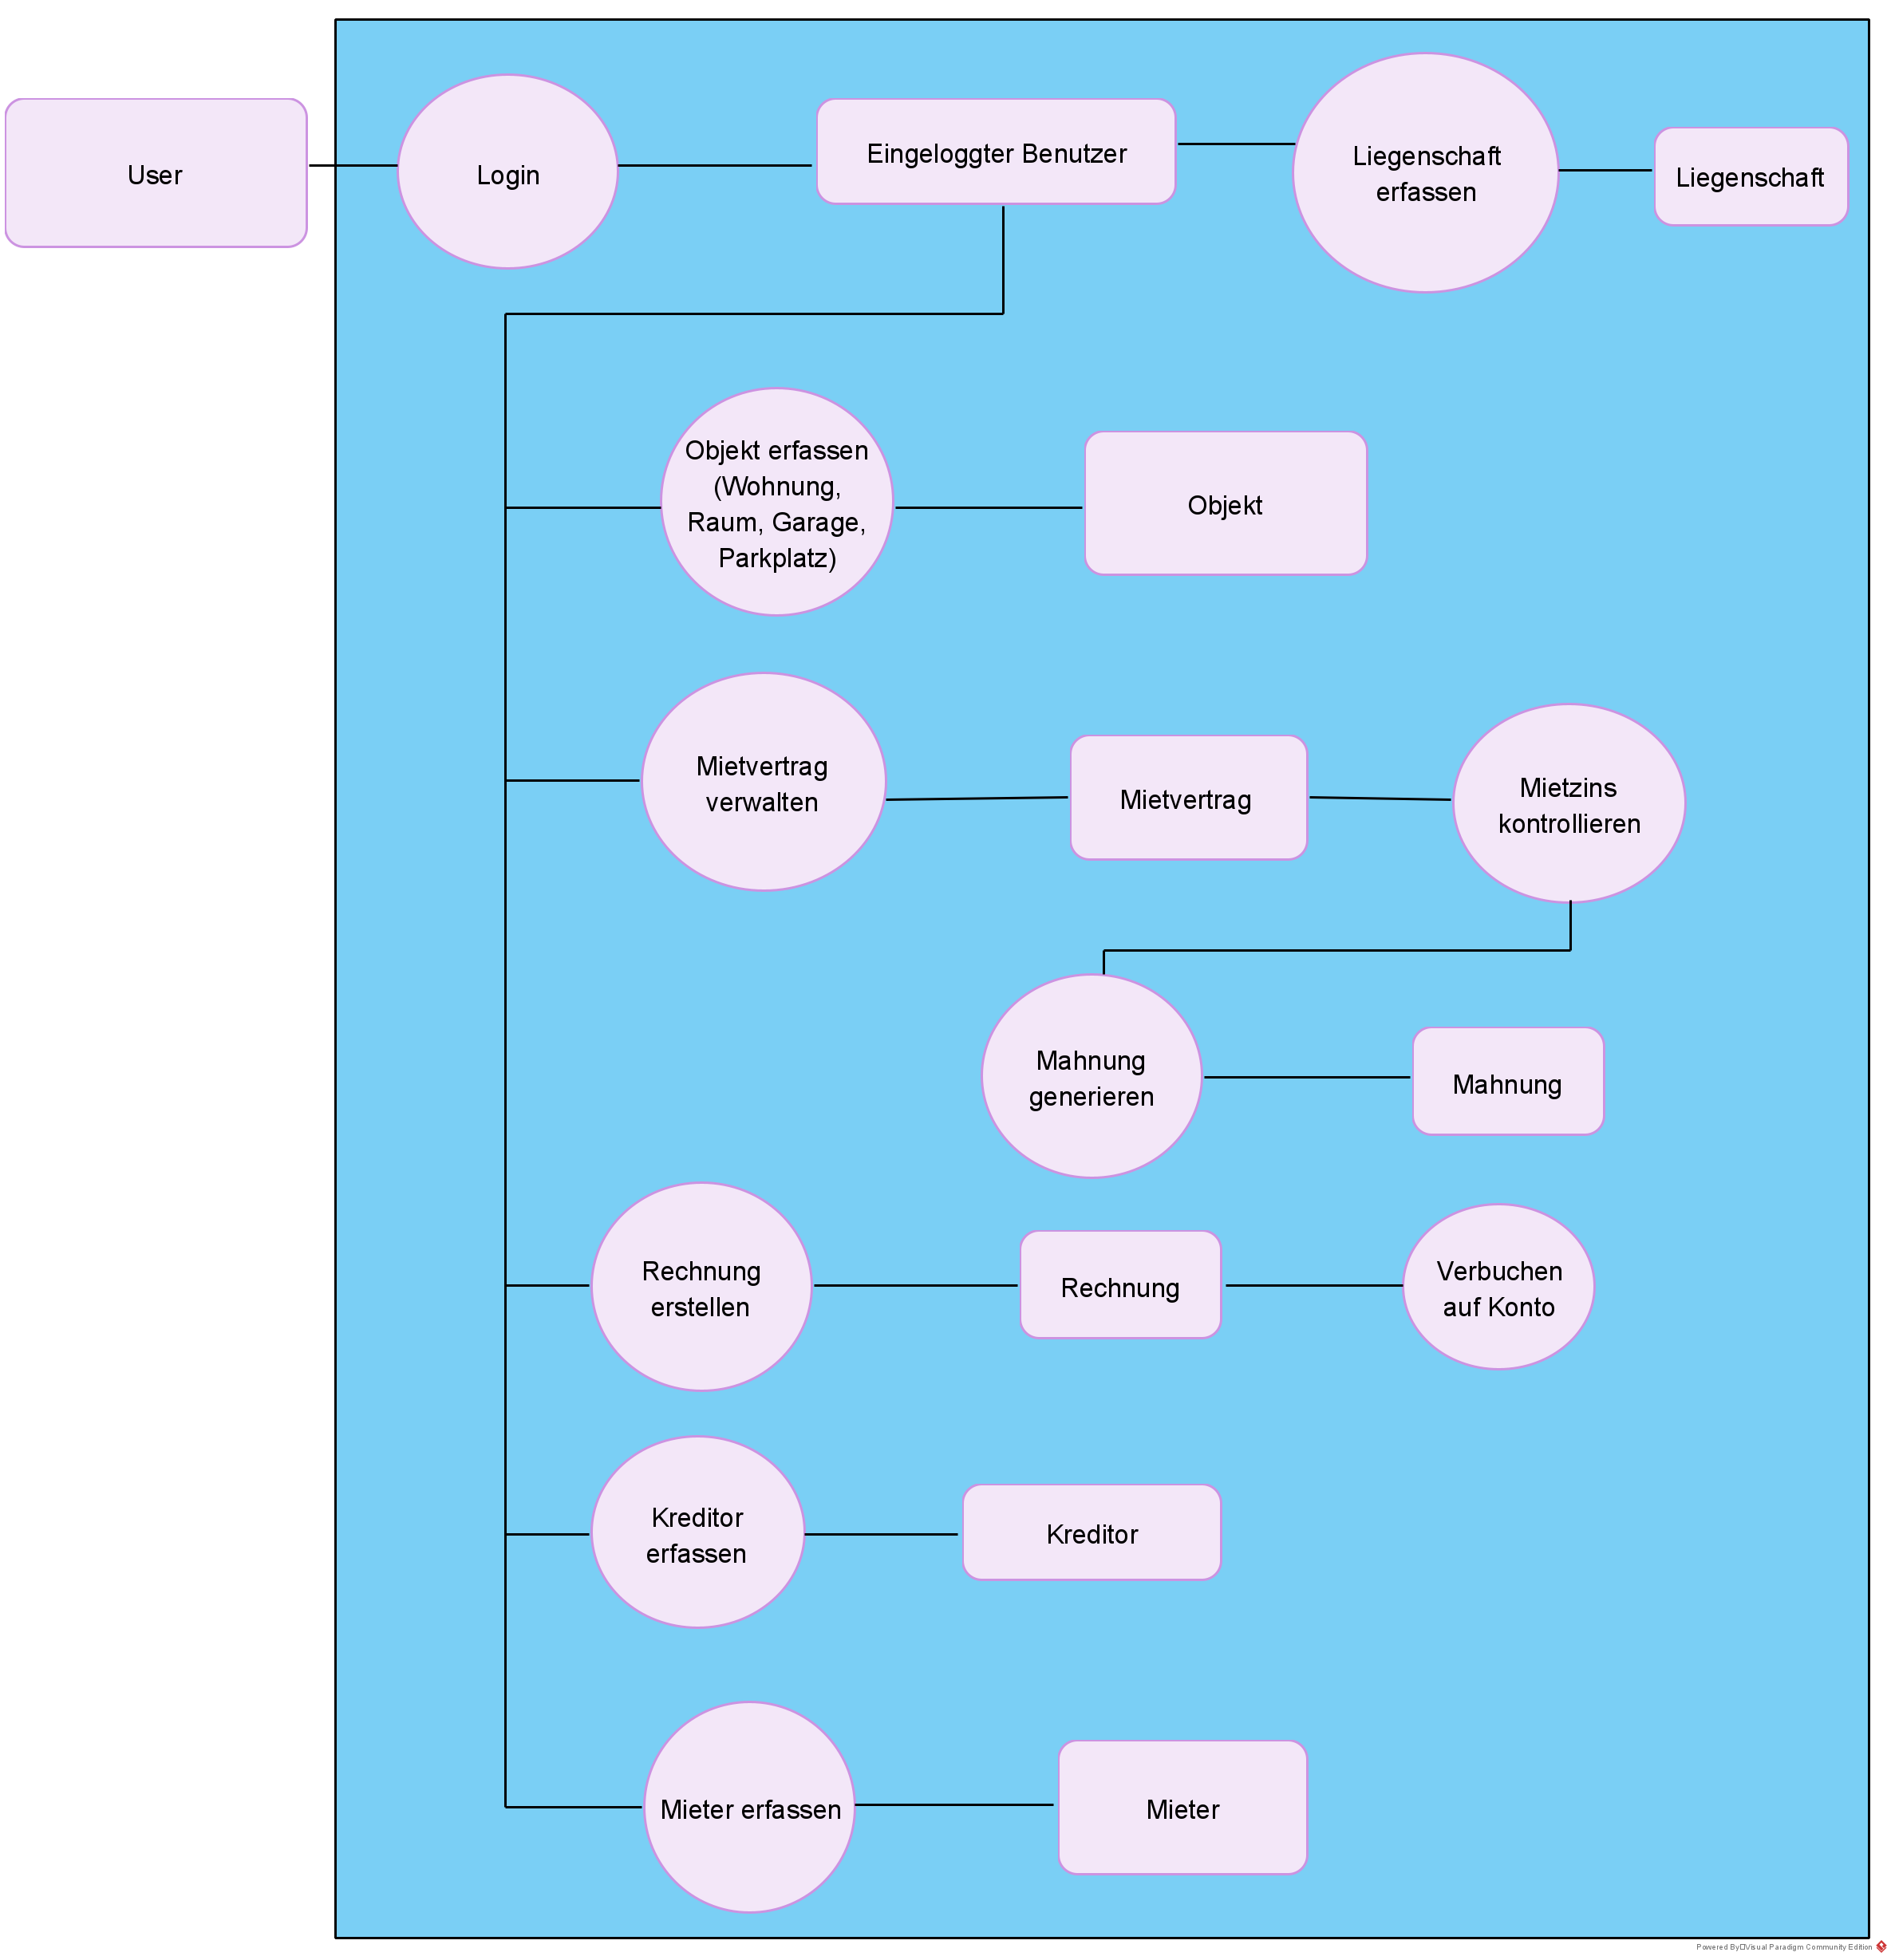
\includegraphics[width=0.99\linewidth]{content/diagrams/out/contextdiagram/context.png}
    \caption{Kontextdiagramm}
  \end{center}
  \label{contextdiag}
\end{figure}

\subsection{Geschäftsprozesse}
\begin{table}[H]
  \newcolumntype{a}{>{\columncolor[HTML]{1EB6FF}}L}
  \centering
  \settowidth\tymin{\textbf{Kurzbeschreibung}}
  \setlength\extrarowheight{2pt}
  \begin{tabulary}{1.0\textwidth}{|a|m{12cm}|}
    \hline
    \textbf{Name}&Liegenschaft erfassen\\
    \hline 
    \textbf{Kurzbeschreibung} & Eine neue Liegenschaft, die die Verwaltung verwaltet, soll hinzugefügt werden. \\
    \hline
    \textbf{Akteure} & Mitarbeiter in der Liegenschaftsverwaltung\\
    \hline
    \textbf{Auslöser} & Die Verwaltung wird mit dem verwalten einer neuen Liegenschaft beauftragt.\\
    \hline
    \textbf{Ergebnis} & Die Liegenschaft ist abgespeichert und werden in der Übersicht angezeigt.\\
    \hline
    \textbf{Eingehende Daten} & Liegenschaft mit allen dazu gehörigen Informationen\\
    \hline
    \textbf{Vorbedingungen} & Die Daten zur Liegenschaft müssen bekannt sein.\\
    \hline
    \textbf{Nachbedingungen} & Keine\\
    \hline
    \textbf{Ablauf} & Der Eingeloggte Mitarbeiter trägt alle Muss-Daten für die neue Liegenschaft ein, und speichert diese. Der Mitarbeiter kann den Objekttyp für die Liegenschaft auswählen und die Informationen pro Objekt eintragen. Wenn der Objekttyp noch nicht erfasst wurde, muss der Objekttyp noch erstellt werden.\\
    \hline
    \textbf{Priorität} & hoch\\
    \hline
  \end{tabulary}
  \caption{GP-Liegenschaft erfassen}
\end{table}

\begin{table}[H]
  \newcolumntype{a}{>{\columncolor[HTML]{1EB6FF}}L}
  \centering
  \settowidth\tymin{\textbf{Kurzbeschreibung}}
  \setlength\extrarowheight{2pt}
  \begin{tabulary}{1.0\textwidth}{|a|m{12cm}|}
    \hline
    \textbf{Name}&Objekt in Liegenschaft erfassen\\
    \hline 
    \textbf{Kurzbeschreibung} & In einer Liegenschaft müssen Objekte hinzugefügt werden \\
    \hline
    \textbf{Akteure} & Mitarbeiter in der Liegenschaftsverwaltung\\
    \hline
    \textbf{Auslöser} & Für die erfasste Liegenschaft wurden noch keine Objekte hinzugefügt\\
    \textbf{Ergebnis} & Objekte sind der Liegenschaft hinzugefügt und in der Übersicht sichtbar\\
    \hline
    \textbf{Eingehende Daten} & Informationen zum erfassenden Objekt\\
    \hline
    \textbf{Vorbedingungen} & Damit ein Objekt zu einer Liegenschaft hinzugefügt werden kann, muss die Liegenschaft erfasst worden sein oder im Erfassungsprozess sein\\
    \hline
    \textbf{Nachbedingungen} & Keine\\
    \hline
    \textbf{Ablauf} & Nach oder während dem Erfassen der Liegenschaft, muss der Benutzer noch die Daten zu den Objekten in der Liegenschaft erfassen. Es müssen alle Informationen zum Objekt angegeben werden und anschliessend abgespeichert werden\\
    \hline
    \textbf{Priorität} & hoch\\
    \hline
  \end{tabulary}
  \caption{GP-Objekt erfassen}
\end{table}

\begin{table}[H]
  \newcolumntype{a}{>{\columncolor[HTML]{1EB6FF}}L}
  \centering
  \settowidth\tymin{\textbf{Kurzbeschreibung}}
  \setlength\extrarowheight{2pt}
  \begin{tabulary}{1.0\textwidth}{|a|m{12cm}|}
    \hline
    \textbf{Name}& Mieter erfassen\\
    \hline 
    \textbf{Kurzbeschreibung} & Neue Mieter sollen in der Applikation hinzugefügt werden\\
    \hline
    \textbf{Akteure} & Mitarbeiter in der Liegenschaftsverwaltung\\
    \hline
    \textbf{Auslöser} & Vermietung eines Objektes an einen neuen Mieter\\
    \hline
    \textbf{Ergebnis} & Ein neuer Mieter wurde in der Applikation erfasst\\
    \hline
    \textbf{Eingehende Daten} & Informationen über den Mieter\\
    \hline
    \textbf{Vorbedingungen} & Die Informationen über den Mieter müssen bekannt sein\\
    \hline
    \textbf{Nachbedingungen} & Keine\\
    \hline
    \textbf{Ablauf} & Der Benutzer der Applikation erstellt einen neuen Mieter. Er gibt alle Informationen ein und speichert den Mieter ab\\
    \hline
    \textbf{Priorität} & hoch\\
    \hline
  \end{tabulary}
  \caption{GA-Mieter Erfassen}
\end{table}

\begin{table}[H]
  \newcolumntype{a}{>{\columncolor[HTML]{1EB6FF}}L}
  \centering
  \settowidth\tymin{\textbf{Kurzbeschreibung}}
  \setlength\extrarowheight{2pt}
  \begin{tabulary}{1.0\textwidth}{|a|m{12cm}|}
    \hline
    \textbf{Name}& Mietvertrag erstellen\\
    \hline 
    \textbf{Kurzbeschreibung} & Es wird ein Mietvertrag für ein Objekt oder eine Liegenschaft erstellt\\
    \hline
    \textbf{Akteure} & Mitarbeiter in der Liegenschaftsverwaltung\\
    \hline
    \textbf{Auslöser} & Neuvermietung eines Objekts oder einer Liegenschaft\\
    \hline
    \textbf{Ergebnis} & Ein Mietvertrag\\
    \hline
    \textbf{Eingehende Daten} & Mieter, Liegenschaft/Objekt, Mietbeginn, Mietzins und Nebenkosten, Informationen zum Mietdepot\\
    \hline
    \textbf{Vorbedingungen} & Das Objekt oder die Liegenschaft und der Mieter muss in der Applikation erfasst worden sein\\
    \hline
    \textbf{Nachbedingungen} & Keine\\
    \hline
    \textbf{Ablauf} & Der Benutzer der Applikation erstellt einen neuen Mietvertrag, indem er alle nötigen Informationen eingibt. Wenn die Informationen vollständig eingegeben wurden, kann ein PDF generiert werden, welches dann von den beiden Parteien unterzeichnet wird \\
    \hline
    \textbf{Priorität} & hoch\\
    \hline
  \end{tabulary}
  \caption{GA-Mietvertrag erstellen}
\end{table}

\begin{table}[H]
  \newcolumntype{a}{>{\columncolor[HTML]{1EB6FF}}L}
  \centering
  \settowidth\tymin{\textbf{Kurzbeschreibung}}
  \setlength\extrarowheight{2pt}
  \begin{tabulary}{1.0\textwidth}{|a|m{12cm}|}
    \hline
    \textbf{Name}& Kreditor erfassen\\
    \hline 
    \textbf{Kurzbeschreibung} & Ein neuer Kreditor wird angelegt\\
    \hline
    \textbf{Akteure} & Mitarbeiter in der Liegenschaftsverwaltung\\
    \hline
    \textbf{Auslöser} & Es wird ein Lieferant, der noch nicht im System ist, mit einer Dienstleistung beauftragt\\
    \hline
    \textbf{Ergebnis} & Ein neuer Kreditor wurde hinzugefügt\\
    \hline
    \textbf{Eingehende Daten} & Informationen über den zu erfassenden Kreditor\\
    \hline
    \textbf{Vorbedingungen} & Es müssen die Informationen über den Kreditor vorhanden sein\\
    \hline
    \textbf{Nachbedingungen} & Keine\\
    \hline
    \textbf{Ablauf} & Der Benutzer erstellt den Kreditor in der Applikation uns Speichert diesen ab\\
    \hline
    \textbf{Priorität} & hoch\\
    \hline
  \end{tabulary}
  \caption{GA-Kreditor erfassen}
\end{table}

\begin{table}[H]
  \newcolumntype{a}{>{\columncolor[HTML]{1EB6FF}}L}
  \centering
  \settowidth\tymin{\textbf{Kurzbeschreibung}}
  \setlength\extrarowheight{2pt}
  \begin{tabulary}{1.0\textwidth}{|a|m{12cm}|}
    \hline
    \textbf{Name}&Rechnung erstellen\\
    \hline 
    \textbf{Kurzbeschreibung} & Eine neue Rechnung erstellen\\
    \hline
    \textbf{Akteure} & Mitarbeiter in der Liegenschaftsverwaltung\\
    \hline
    \textbf{Auslöser} & Es wurde eine Dienstleistung, die die Liegenschaftsverwaltung getätigt hat, bezogen \newline 
    Für eine Liegenschaft oder ein Objekt wurde die Nebenkostenabrechnung erstellt\\
    \hline
    \textbf{Ergebnis} & Eine Rechnung\\
    \hline
    \textbf{Eingehende Daten} & Informationen warum die Rechnung erstellt werden muss \\
    \hline
    \textbf{Vorbedingungen} & Keine\\
    \hline
    \textbf{Nachbedingungen} & Keine\\
    \hline
    \textbf{Ablauf} & Der Benutzer erstellt eine neue Rechnung und gibt alle nötigen Informationen für die Rechnung ein.\\
    \hline
    \textbf{Priorität} & hoch\\
    \hline
  \end{tabulary}
  \caption{GA-Rechnung erstellen}
\end{table}

\begin{table}[H]
  \newcolumntype{a}{>{\columncolor[HTML]{1EB6FF}}L}
  \centering
  \settowidth\tymin{\textbf{Kurzbeschreibung}}
  \setlength\extrarowheight{2pt}
  \begin{tabulary}{1.0\textwidth}{|a|m{12cm}|}
    \hline
    \textbf{Name}&Mietzinskontrolle\\
    \hline 
    \textbf{Kurzbeschreibung} & Es muss überprüft werden, ob der betreffende Mietzins schon bezahlt wurde \\
    \hline
    \textbf{Akteure} & Mitarbeiter in der Liegenschaftsverwaltung\\
    \hline
    \textbf{Auslöser} & Mietzinszahlungsüberprüfung\\
    \hline
    \textbf{Ergebnis} & Bei negativer Prüfung eine Mahnung\newline 
    Bei positiver Prüfung nichts\\
    \hline
    \textbf{Eingehende Daten} & keine\\
    \hline
    \textbf{Vorbedingungen} & Es müssen Mietverträge im System erfasst sein\\
    \hline
    \textbf{Nachbedingungen} & Keine \\
    \hline
    \textbf{Ablauf} & Der Benutzer überprüft ob für ein entsprechendes Objekte/Liegenschaft die Miete bezahlt wurde. Wenn die Miete noch nicht bezahlt wurde, kann er direkt eine vorgefertigte Mahnung generieren und ausdrucken.\\
    \hline
    \textbf{Priorität} & hoch\\
    \hline
  \end{tabulary}
  \caption{GA-Mietzinskontrolle}
\end{table}